\documentclass[onecolumn, draftclsnofoot,10pt, compsoc]{IEEEtran}
\usepackage{graphicx}
\usepackage{url}
\usepackage{setspace}

\usepackage{geometry}
\geometry{textheight=9.5in, textwidth=7in}

% 1. Fill in these details
\def \CapstoneTeamName{			Velocity-Raptors}
\def \CapstoneTeamNumber{		37}
\def \GroupMemberOne{			Alex Bailey}
\def \GroupMemberTwo{			Dylan Washburne}
\def \GroupMemberThree{			Benjamin Wick}
\def \CapstoneProjectName{		Object Velocity Tracking}
\def \CapstoneSponsorCompany{}
\def \CapstoneSponsorPerson{		Alex Neighbors}

% 2. Uncomment the appropriate line below so that the document type works
\def \DocType{		%Problem Statement
				%Requirements Document
				%Technology Review
				%Design Document
				Progress Report
				}
			
\newcommand{\NameSigPair}[1]{\par
\makebox[2.75in][r]{#1} \hfil 	\makebox[3.25in]{\makebox[2.25in]{\hrulefill} \hfill		\makebox[.75in]{\hrulefill}}
\par\vspace{-12pt} \textit{\tiny\noindent
\makebox[2.75in]{} \hfil		\makebox[3.25in]{\makebox[2.25in][r]{Signature} \hfill	\makebox[.75in][r]{Date}}}}
% 3. If the document is not to be signed, uncomment the RENEWcommand below
%\renewcommand{\NameSigPair}[1]{#1}

%%%%%%%%%%%%%%%%%%%%%%%%%%%%%%%%%%%%%%%
\begin{document}
\begin{titlepage}
    \pagenumbering{gobble}
    \begin{singlespace}
    	
\includegraphics[height=4cm]{coe_v_spot1}
        \hfill 
        % 4. If you have a logo, use this includegraphics command to put it on the coversheet.
        %\includegraphics[height=4cm]{CompanyLogo}   
        \par\vspace{.2in}
        \centering
        \scshape{
            \huge CS Capstone \DocType \par
            {\large\today}\par
            \vspace{.5in}
            \textbf{\Huge\CapstoneProjectName}\par
            \vfill
            {\large Prepared for}\par
            \Huge \CapstoneSponsorCompany\par
            \vspace{5pt}
            {\Large\NameSigPair{\CapstoneSponsorPerson}\par}
            {\large Prepared by }\par
            Group\CapstoneTeamNumber\par
            % 5. comment out the line below this one if you do not wish to name your team
            %\CapstoneTeamName\par 
            \vspace{5pt}
            {\Large
                \NameSigPair{\GroupMemberOne}\par
                \NameSigPair{\GroupMemberTwo}\par
                \NameSigPair{\GroupMemberThree}\par
            }
            \vspace{20pt}
        }
        \begin{abstract}
        % 6. Fill in your abstract    
        	This document is intended to give an update for the progress of our project.
            It includes goals, project status, pieces of interesting code to share, problems, and weekly updates.
            
        \end{abstract}     
    \end{singlespace}
\end{titlepage}
\newpage
\pagenumbering{arabic}
\tableofcontents
% 7. uncomment this (if applicable). Consider adding a page break.
%\listoffigures
%\listoftables
\clearpage

% 8. now you write!
\section{Project Purpose and Goals (Benjamin Wick)}
The overall purpose of our project is to use a stationary camera to detect moving objects and then determine the velocity at which the objects are moving to output the speed of the object.
This project is intended to be a proof of theory where future larger scaled systems can then be implemented based off our smaller scaled project.
In theory, the objects can be anything the user wishes to track which can include, but not limited to, vehicles, people, sports objects, animals and any other moving objects the user wishes to track.
There can be many different applications over many different fields for this kind of system.
An example is using the system to monitor the average speed at which cars are traveling on the freeway.
This system can be implemented using different cameras and hardware to meet the needs of the user.
In the case of our project, we will use a Microsoft Kinect to track the motion of an object, such as people or RC cars, and determine the velocity at which they are moving.

The goal of our project is to create a working prototype with a friendly user interface in the form of a Microsoft Windows application which will display the video feed and speed.
Accuracy and reliability is another goal important goal we intend to accomplish.
We intend to be able to track a person and their velocity at an accuracy of 90\% of their true velocity.

\section{Current Status of Project (Alex Bailey)}
\subsection{Fall Status}
Currently we have all needed written documents to begin our project.
This includes a requirements document, a technology review, and an overall design document.
We currently have not started on the implementation of our project.
We have done enough research to begin implementation.
The next order of business is to choose a camera system that will enable us to begin coding.

\subsection{Winter Midterm Status}
Our current project status is that we are beginning implementation while continuing research for our project.

For our Graphical User Interface (GUI) we have a basic design, with a menu bar at the top, a box for viewing the camera, and a start button. The menu bar is currently only a skeleton, with it's feature not implemented yet. 
Our GUI does allow the user to select their web camera, or any other recognized camera, from a drop down menu and have the feed displayed live on the screen.

For our camera our client has supplied a Kinect from the Xbox 360 for us to use. 
The Kinect is slightly different than the types of cameras that we had originally planned to use.
The Kinect is not a stereoscopic camera in the sense that it uses two cameras in order to determine how far away a given object is. 
The Kinect instead uses an infrared projector to display a pattern of dots onto the surfaces in front of it that an infrared camera is then capable of detecting and uses those dots to make a depth map for distance tracking.
The Kinect also contains a color camera. 
We are currently researching the Kinect's API in order to display the color camera on screen as well as access the depth map for distance tracking purposes.

We are looking at how to use OpenCV and C\# in order to implement the image subtraction method.
We are also considering how to best include the depth map provided by the Kinect in the object tracking process as we did not take it into consideration when examining the tracking methods. 
We are also looking into more human recognition programs to determine if working with people might be simpler and if we do it may be more effective to use software like this as opposed to relying entirely on image subtraction.

\section{Work Remaining (Dylan Washburne)}
Basic functionality is still required for both testing and standard use.  Boxes around identified objects will allow for easier debugging and confirmation that an object is properly oriented in the scene.  Returning numbers to the screen will allow for high-precision identification of an object's recognized position, and can be later re-purposed for displaying each object's velocity.

We hope to expand upon the rather basic functionality we are currently gaining from the Kinect's object tracking.  
Our intents include the following design points: the ability track multiple objects simultaneously, calculating the velocity of all objects getting tracked, and recording all the velocity data to a server, for later statistical use.

We hope to update the user interface part of the design.  Features we wish to include involve allowing the user to start and stop the recording with the click of a single button, and the ability to playback previous recordings.  

\section{Problems (Dylan Washburne)}
During the first term, we did not run into any major issues.
This stems from the fact the first term, we were mostly working on documentation on the process.
We were rather good at this process, so major issues never really cropped up.

During the second term, we had issues in the acquisition of our camera.  
We made our request for a camera on the first week of the term, but it took several weeks to arrive.
Alongside that, we had requested a specific camera known as a ZED, however what was sent to us was a Microsoft Kinect.
This caused us to contact our client about the issue and he confirmed that this was intentional.
We were from there able to reorient ourselves to work with the Kinect. 
That said, the combination of the camera not arriving for several weeks and not being the model we had researched and prepared for caused a large turnaround time while we scrambled to work with our suboptimal scenario.

\section{Pieces of Code}
We do not feel any of the code we have created is unique and special enough to be worth sharing at this time.

\section{Hardware (Benjamin Wick)}
We chose to use the Microsoft Xbox 360 Kinect. The Kinect has an RGB camera as well as two 3D depth sensors. These depth sensors should help us create a depth map that can be used to determine the distance of a person on the screen, which will be vital in determining speed.
\newline
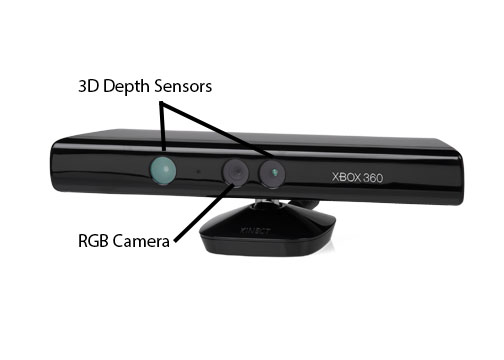
\includegraphics[height=5.5cm]{kinect1}
\newline
The Kinect was made for the Xbox 360 which meant we had to buy an adapter that will allow us to plug it into a female USB port. Below is an image of the adapter that will be used to do so.
\newline
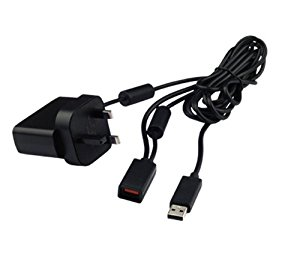
\includegraphics[height=5.5cm]{adapter}
\newline
Both these hardware components aren't necessary for every system to be implemented.
Theoretically, other cameras may be used depending on the object being tracked.
We chose to use the Kinect because of price, convenience, and the ability to detect people.
The combination of these two hardware pieces will allow us to create a live video for our program to detect objects which will help us obtain our goal.



\section{Retrospective}

\subsection{Fall Term}

\subsubsection{Weeks 1-3}
In weeks 1-3 we contacted our client, Alex Neighbors and spoke to him about what he wanted the project to be and how he wanted it to be done.
We also wrote the Problem Statement, a document to define and describe our projects problem.
\subsubsection{Week 4}
In week 4 we revised our problem statement, we needed help making sure that it was acceptable so we asked our TA, Jon Dodge, and he gave us good feedback 
\subsubsection{Week 5}
In week 5 we completed our final draft of our problem statement and turned it in.
We discussed the use of different cameras and which would be our best option.
However since the camera we pick has a big impact on our project, we need to do further research.
\subsubsection{Week 6}
In week 6 we worked our requirements document.
We received feedback from John Dodge and Professor Kirsten Winters.
We sent our Alex Neighbors our requirements document so that he could give us his comments and approval.
\subsubsection{Week 7}
In week 7 we completed our requirements document, got approval, and turned it in.
We also began work on the Tech Review by discussing its requirements.
\subsubsection{Week 8}
In week 8 we research the technologies for our tech review and wrote the tech review.
\subsubsection{Week 9}
In week 9 we started to work on our design document.
This document is important because it would help lead us on when we begin implementation of our project.
We did not run into any major issues while working on it.
\subsubsection{Week 10}
In week 10 we wrote and turned in the design document.
We did not obtain a signature on it before the due date, but an email from Kirsten indicated that we could turn in what we had and obtain the signature later.
We took this option to successfully turn in the design document on time.

\subsection{Winter Term}

\subsubsection{Week 1 (Benjamin Wick) }
This week was the first week of winter term. It was also our first meeting since fall term. We met up to begin researching the camera to request. We talked about what days we should meet up to set a schedule.

\subsubsection{Week 2 (Dylan Washburne) }
On this week, we finished our research on potential cameras to use for the project.  We sent our client a request to purchase the camera for us. 

\subsubsection{Week 3 (Dylan Washburne) }
A mostly uneventful week.  We sent our client additional emails to ensure we would receive the camera in a timely manner.  We continued our work on creating an interface while we waited.

\subsubsection{Week 4 (Dylan Washburne) }
The camera arrived this week.  Instead of the brand we had proposed in email 2 weeks prior, it was instead a Kinect.  We made contact with our client to discuss this, and were informed the camera selection was an intentional choice.

From here, we redefined our project's scope to fall in-line with the more limited parameters of the Kinect.  We have determined the project is a proof-of-concept, and will update our documentation to reflect our new scope.

\subsubsection{Week 5 (Dylan Washburne) }
Recieved a usb adapter which will allow us to interact directly with the Kinect.  Set up the environment to program the project in.

\subsubsection{Week 6 (Dylan Washburne)}
Updated documents to reflect the specifications of the Kinect.  Did further work understanding the basics of the Kinect's usage.  Created midterm progress report and presentation.

\subsection{Retrospective Table}

\begin{tabular}{|p{0.3\linewidth} |p{0.3\linewidth}|p{0.3\linewidth}|}
\hline 
 Fall Term & & \\
\hline 
Positives & Deltas & Actions \\
\hline
We finished all the papers & - & - \\
\hline
- & We need to select a camera & Research and select a camera \\
\hline


\end{tabular}

\begin{tabular}{|p{0.3\linewidth} |p{0.3\linewidth}|p{0.3\linewidth}|}
\hline 
Winter Term & & \\
\hline 
Positives & Deltas & Actions \\
\hline
Documents have been updated & - & - \\
\hline
Created a User Interface & - & - \\
\hline
Gathered all required hardware & - & - \\
\hline
Gained more insight and knowledge of our project through research & - & - \\
\hline
Able to stream a live video feed using a camera & - & - \\
\hline
- & Need to begin tracking objects & Research how to use OpenCv and track objects \\
\hline
- & Need to begin calculating speed & Research methods and algorithms that may help us calculate object speeds \\
\hline
- & Not meeting often & meet multiple times a week in order to be on the same page and discuss issues face to face \\
\hline
- & Not very clear objectives & Either use a method of production like Agile or have set goals. \\
\hline
- & Miscommunication about project goals & Be more specific and keep in contact more with client. \\
\hline
\end{tabular}

\end{document}